%-----------------------------------------------------------------------------------%
\section{The Detector}\label{sec:THE_hawc}
%-----------------------------------------------------------------------------------%

\begin{figure}[h!]
    \centering{
    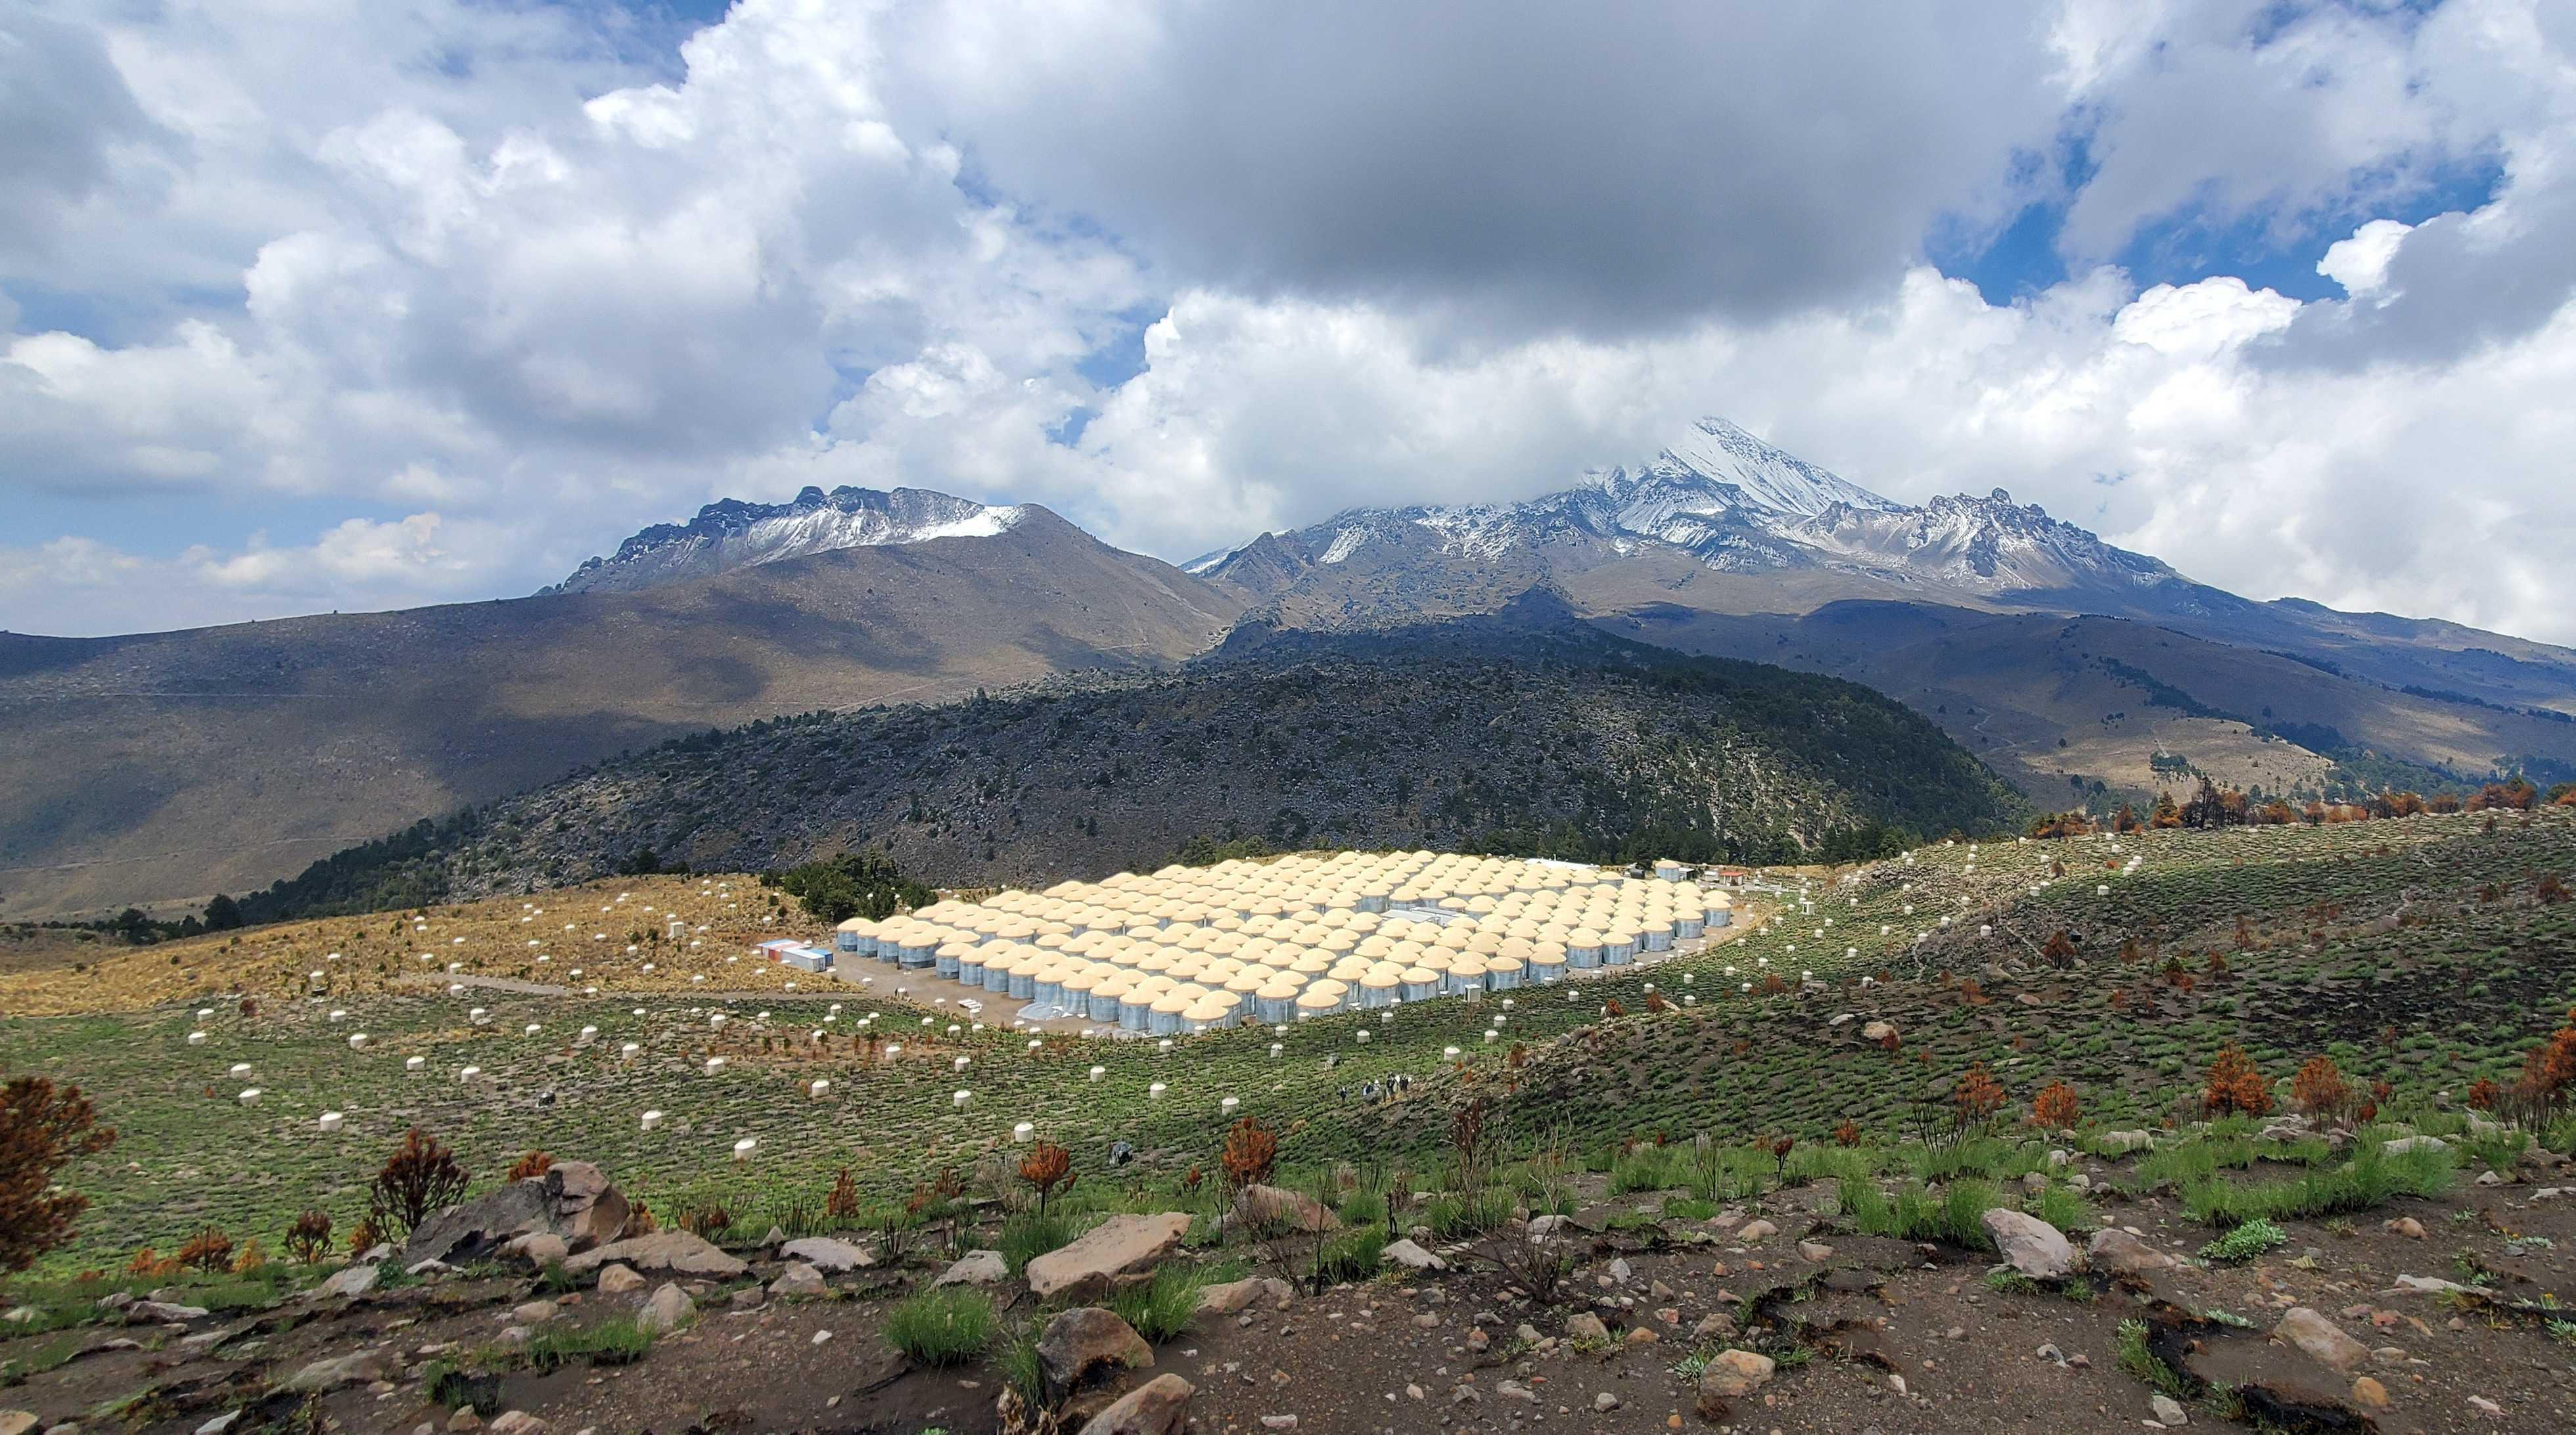
\includegraphics[scale=0.155]{figures/hawc/HAWC.jpg}
    }
    \caption{Photo of the HAWC detector that I took on May 17, 2023. Main array is centered in the photo and comprised of the larger tanks. Outriggers are the smaller tanks around the main array.}
    \label{fig:HAWC}
\end{figure}

The High Altitude Water Cherenkov (HAWC) Observatory is a specialized instrument designed for the observation of high energy gamma-rays and cosmic rays \cite{HAWC_NIM}.
Located on the Sierra Negra volcano in Mexico, HAWC observes gamma rays and cosmic rays in the energy range of approximately 100 GeV to 100'ss of TeV.
HAWC is strategically situated to maximize observational efficiency due to its high altitude.
At an elevation of 4,100 meters, it monitors about two-thirds of the sky every day with an uptime above 90\%.
This capability is essential for studying high-energy astronomical phenomena.

HAWC comprises of 300 water Cherenkov detectors (WCDs) spread over 22,000 square meters.
Each main array detector is filled with purified water and equipped with four, upward-facing photomultiplier tubes (PMTs).
These PMTs detect Cherenkov radiation from charged particles passing through the tanks.
These charged particles are generated when a high energy gamma or cosmic ray collides with gas in the atmosphere to create a charged particle shower, see \cref{fig:airshowers}.
The observatory includes a separate tank configuration which are refered to as the outriggers.
They are a secondary array of 345 smaller WCD's.
Surrounding the main array, each outrigger tank measures 1.55 meters in diameter and height and contain a single upward-facing eight-inch PMT.
This expansion increases the instrumented footprint fourfold.
It improves the reconstruction of showers extending beyond the main array, especially for events above 10 TeV.
However, at the time of writing this thesis, the outriggers have not been fully integrated into HAWC's reconstruction software.

\begin{figure}
    \centering{
    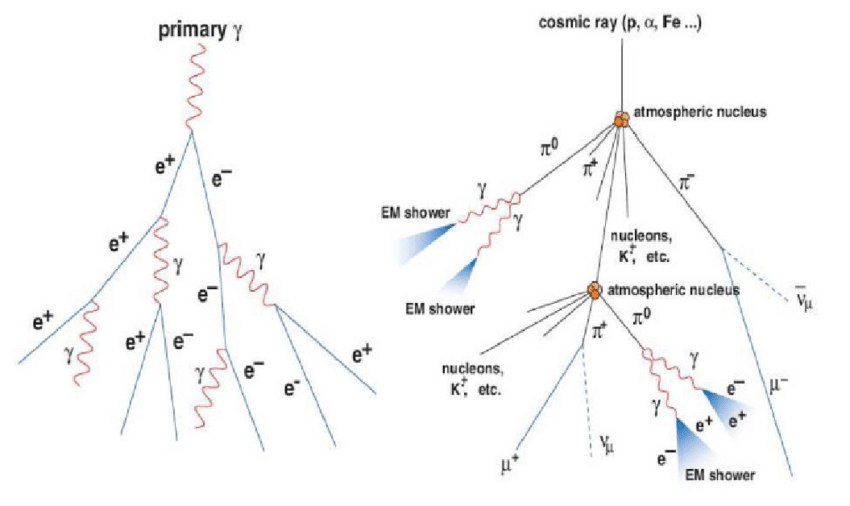
\includegraphics[scale=0.5]{figures/hawc/high_energy_air_shower.png}
    }
    \caption{A particle physics illustration of high energy particle showers. Left shower is an electromagnetic shower from a high energy gamma-ray. Most particles in the shower will be a combination of photons and charged leptons, in this case electrons (e). Right figure shows a cosmic ray particle shower. The cosmic ray will produce many more types of particles including pions ($\pi$), neutrinos, and charged leptons. Figured pulled from \cite{lopez_thesis}.}
    \label{fig:airshowers}
\end{figure}

%-----------------------------------------------------------------------------------%
\subsection{Construction and Hardware} \label{sec:hawc_hardware}
%-----------------------------------------------------------------------------------%

\begin{figure}
    \centering{
        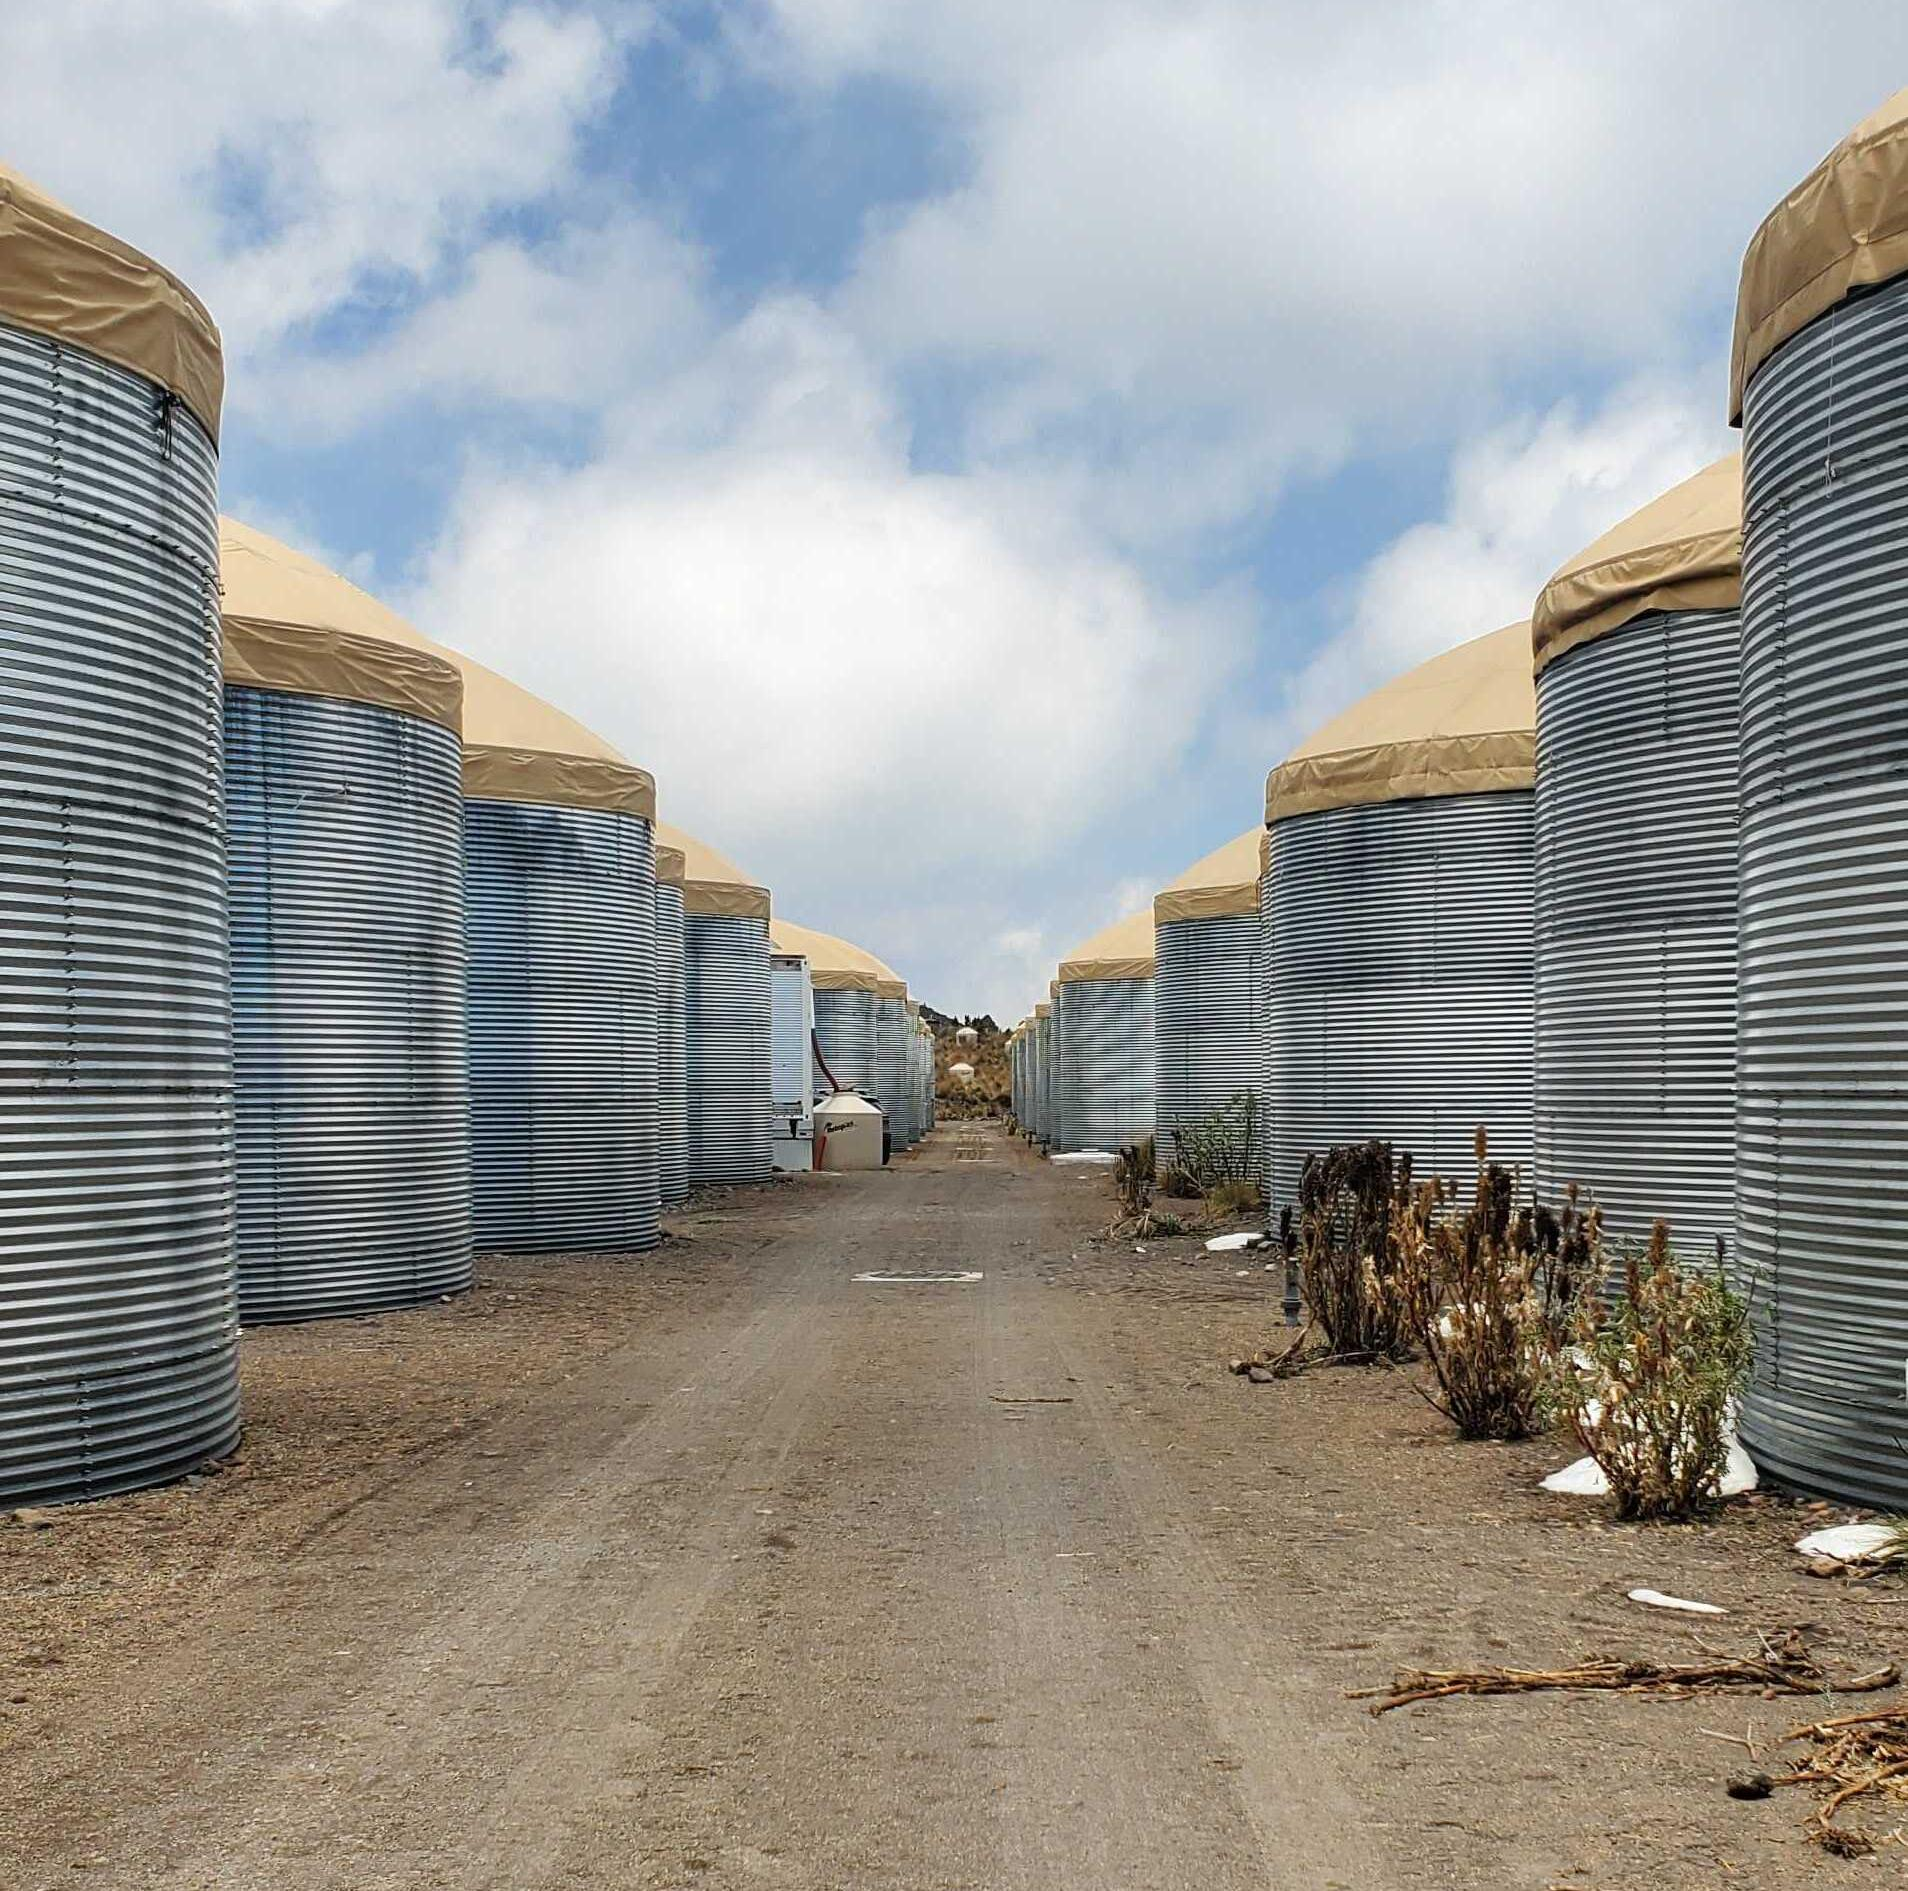
\includegraphics[scale=0.14]{figures/hawc/WCDs.jpg}
        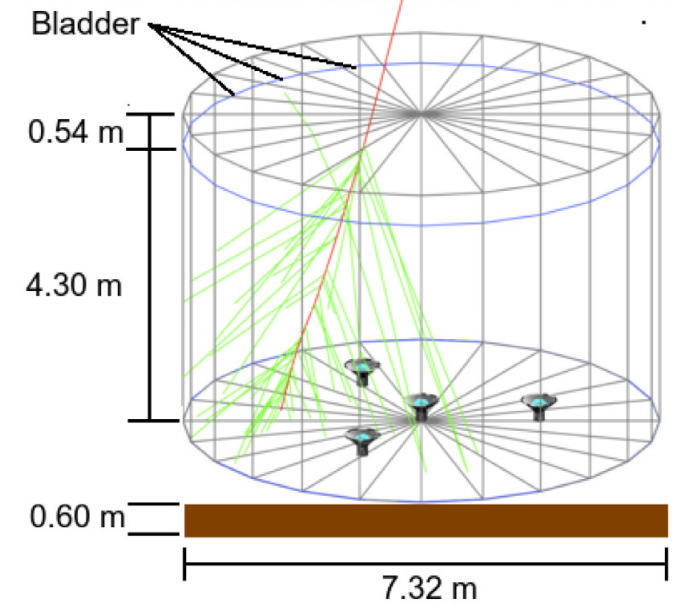
\includegraphics[scale=0.45]{figures/hawc/WCD_schematic.png}
    }
    \caption{The WCDs. Left image features several WCDs looking from within the main array of HAWC. Right image shows a schematic of a WCD pulled from \cite{HAWC_NIM}.}
    \label{fig:WCD_schematic}
\end{figure}
\todo{fact check the content below. GPT may have hallucinated}
Each main array WCD is a cylindrical tank with dimensions of 7.3 m in diameter and 5.4 m in height and filled with 180,000 liters of water \cite{HAWC_NIM}.
The metal shell of these tanks is made from bolted together, corrugated, galvanized steel panels.
The tanks are placed into 0.6 m deep trenches filled with rammed earth to secure it against seismic activity.
The interior of each tank is lined with a black, low-density polyethylene bladder, designed to be impermeable to external light and to prevent reflection of Cherenkov light within the tank.
This bladder is approximately 0.4 mm thick and composed of two layers of three-substrate film.
To further minimize light penetration, a black agricultural foil covers the bladder.
The ground and walls inside the tank are protected with felt and sand to safeguard against punctures.
The tanks are filled 4.5 m deep of purified water, achieving a photon attenuation length for Cherenkov photons that exceeds the tank's dimensions.
This purification level ensures the optimal detection environment for the photons generated by traversing charged particles.

At the base of each tank, four photomultiplier tubes (PMTs) are installed to detect the Cherenkov radiation emitted by charged particles.
Three 8-inch diameter PMTs surround a larger 10 inch PMT from Hamamatsu \cite{hawc_pmt}.
The variation in PMT response is carefully accounted for in event reconstruction algorithms.
Signals from the PMTs travel  610 ft cables to the counting house, where they are processed by Front-End Boards (FEBs).
These FEBs, along with Time to Digital Converters (TDCs), digitize the signals and manage the high voltage supply to the PMTs.

%-----------------------------------------------------------------------------------%
\subsection{Data Acquisition and Signal Processing} \label{sec:hawc_daq}
%-----------------------------------------------------------------------------------%

\begin{figure}
    \centering{
        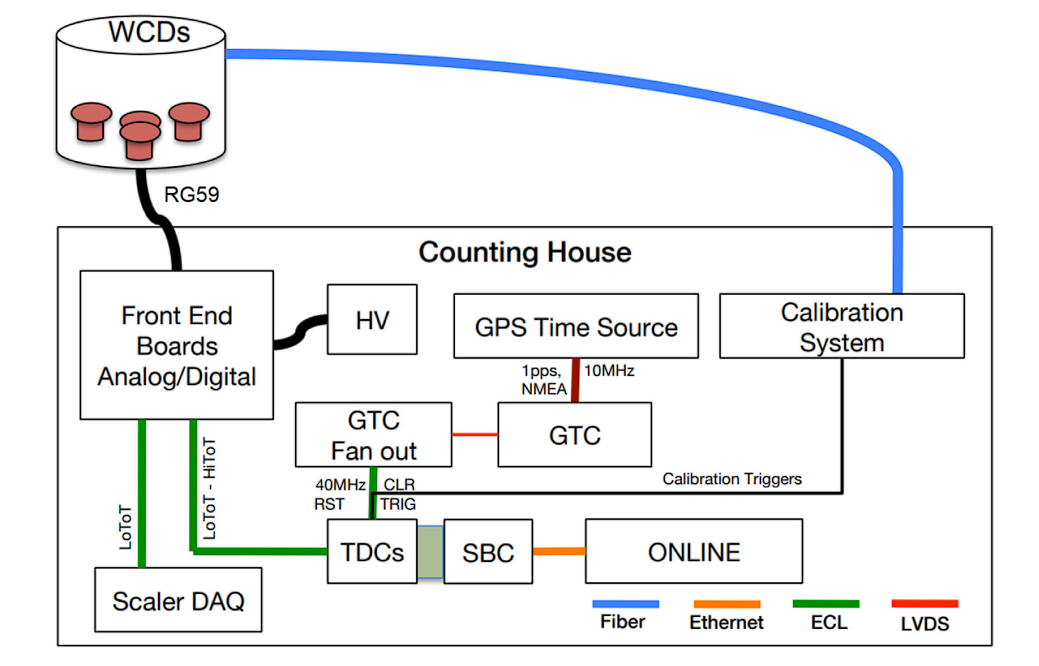
\includegraphics[scale=0.5]{figures/hawc/tank_basic_schem.png}
    }
    \caption{\todo{copied from nim}. Top-level diagram of the HAWC electronics showing a summary of the critical subsystems and the interconnections, including HV and optical fiber cabling. NMEA refers to the National Marine Electric Association format in which GPS presents data [66,67]; CLR, TRG and RST are control signals for the TDC system. The LoToT andHiToT time over threshold signals are discussed in Section 4.1}
    \label{fig:basic_tanks_schem}
\end{figure}

\begin{figure}
    \centering{
        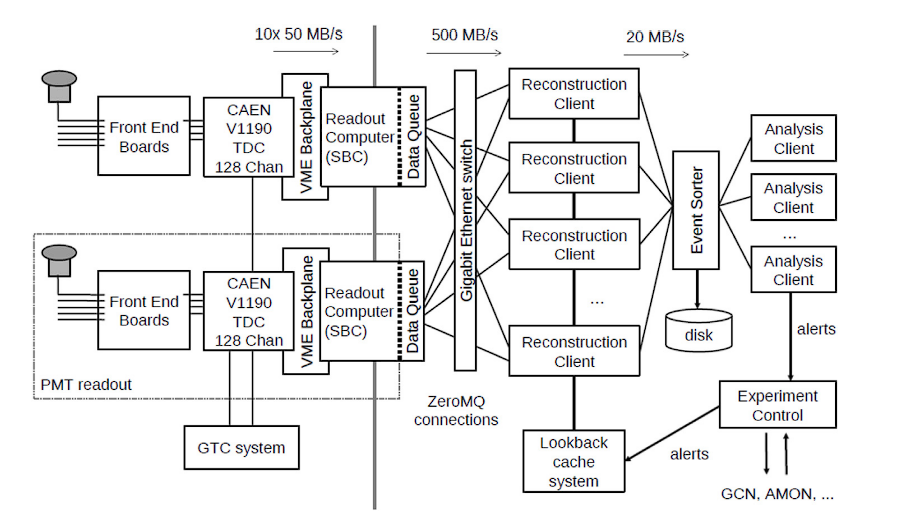
\includegraphics[scale=0.6]{figures/hawc/digital_schematic.png}
    }
    \caption{\todo{copied from NIM}. Schematic overview [68] of the HAWC data acquisition and online processing system, as described in the text of Section 4}
    \label{fig:dig_schem}
\end{figure}

The HAWC data acquisition (DAQ) and signal processing systems convert the physical detection of particles into analyzable data.
This process involves a series of steps from initial signal detection by PMTs to digital conversion and preliminary analysis, see \cref{fig:basic_tanks_schem} and \cref{fig:dig_schem}.

\begin{figure}
    \centering{
        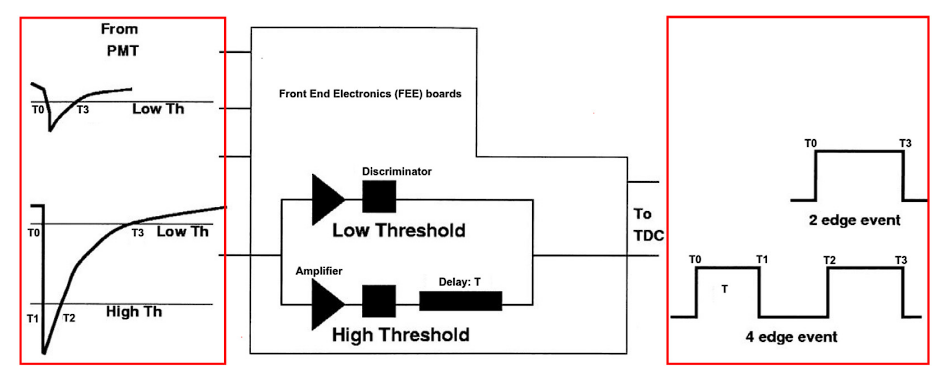
\includegraphics[scale=0.6]{figures/hawc/ToT_threshold.png}
    }
    \caption{\todo{text copied from nim}. The analog PMT signals are split and passed through two paths. In each path, there is an amplifier and discriminator circuit. The ratio of the amplifier gains is 7 to 1. The higher gain circuit has an effectively lower threshold (Low Th). There is a time (T) delay in the high threshold (High Th) path. The 2-edge event is related with the Low Th, while the 4 edge event is related to the High Th.}
    \label{fig:tot_threholds}
\end{figure}

Once the signal from the PMTs arrive at the counting house, they enter the Front-End Boards (FEBs).
The FEBs are responsible for the initial processing of these signals, which includes amplification and integration \cite{Milagro_DAQ}.
Each PMT signal is compared against preset LOW/HIGH voltage thresholds in the FEBs \cref{fig:tot_threholds}, identifying signals that correspond to about 1/4 and 4 photoelectrons, respectively.
This differentiation allows the system to gauge the strength of the detected Cherenkov radiation.
The processed signals are then digitized by Time to Digital Converters (TDCs).
These converters measure the time over threshold (ToT) for each signal, a parameter that reflects both the duration and amplitude of the signal.
This digitization facilitates reconstruction of the original event for translating the physical interactions within the detectors into data \cite{nim:hawc_detect,HAWC_DAQ_NIM,Milagro_DAQ}.

Synchronization across the HAWC observatory is maintained by a central GPS Timing and Control (GTC) system, which achieves a timing resolution of 98 ps.
This high-resolution timing is vital for accurately reconstructing the timing and location of air showers initiated by cosmic and gamma rays.
The GTC system ensures that all components of the DAQ operate in unison to preserve the temporal integrity of the detected events \cite{nim:hawc_detect,hawc_daq_thesis}.

Once digitized, the data are transferred to an online event reconstruction system.
This system runs the Reconstruction Client, which utilizes the raw PMT data to reconstruct the characteristics of the air showers, such as their direction and energy \cite{HAWC_DAQ_NIM}.
The capacity for real-time analysis allows HAWC to promptly respond to astrophysical phenomena like Gamma Ray Bursts (GRBs) and to participate in multi-messenger astronomy by following up on alerts from other observatories.
This real-time processing system is designed to handle high data throughput, using ZeroMQ \cite{zeromq} for efficient data transfer between software components.
Analysis Clients perform specific online analyses that require immediate data, including monitoring for GRBs, solar flare activity, and participation in global efforts to track gravitational waves and neutrinos \cite{nim:hawc_detect}.

The DAQ system is overseen by an Experiment Control system and crew that manage the operational aspects of data collection.
This includes initiating and terminating data collection runs and monitoring the experiment for errors.
In the event of a system crash, often caused by environmental factors such as lightning, the Experiment Control system is designed to automatically restart the experiment and minimize downtime \cite{nim:hawc_detect,HAWC_DAQ_NIM}.

%-----------------------------------------------------------------------------------%
\section{Events Reconstruction} \label{sec:hawc_reconstruction}
%-----------------------------------------------------------------------------------%

Event reconstruction at the HAWC Observatory is a critical procedure that converts the raw data from the observatory's WCDs into a coherent framework for understanding cosmic and gamma-ray events.
This process includes several distinct steps.
Core Fitting determines the geometric center of the air shower on the detector plane.
Angle Reconstruction assesses the trajectory of the incoming particle, revealing its origin in the sky.
Energy Estimation is performed using both \textit{f}-hit and Neural Network (NN) methods to quantify the energy of the detected events.
Gamma-hadron (G\H) discrimination differentiates between gamma-ray and hadronic cosmic ray initiated showers, a vital step for astrophysical interpretations.
Each of these steps is integral to the observatory's objective of investigating the high-energy universe and enable the transformation of signals into detailed insights about high energy cosmic phenomena.

%$$$$$$$$$$$$$$$$$$$$$$$$$$$$$$$$$$$$$$$$$$$$$$$$$$$$$$$$$$$$$$$$$$$$$$$$$$$$$$$$$$$%
\subsection{Core Fitting} \label{sec:hawc_core_fitting}
%$$$$$$$$$$$$$$$$$$$$$$$$$$$$$$$$$$$$$$$$$$$$$$$$$$$$$$$$$$$$$$$$$$$$$$$$$$$$$$$$$$$%

\begin{figure}[h!]
    \centering{
    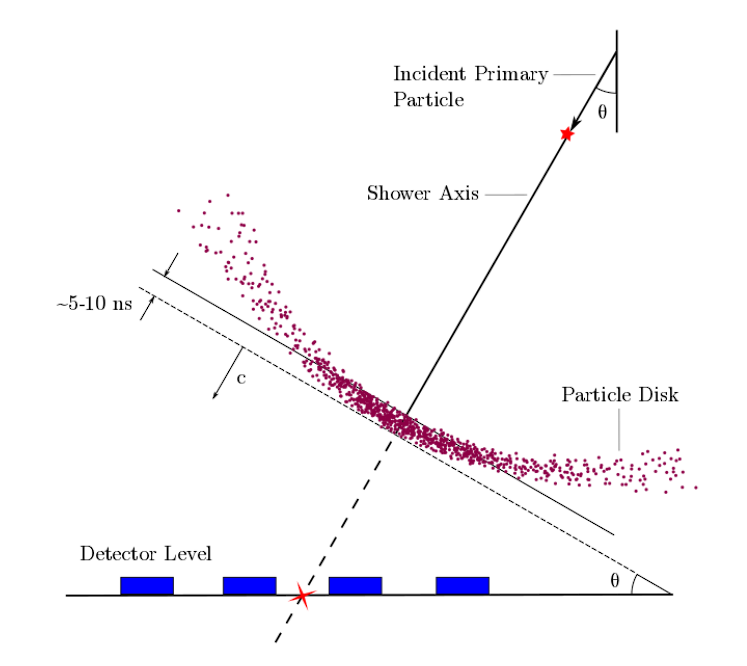
\includegraphics[scale=0.5]{figures/hawc/shower_shape.png}
    }
    \caption{\todo{copied from A's thesis}. An illustration of the angle reconstruction of the original particle. The secondary particles of an air shower travel in a plane perpendicular to the direction of the original particle, allowing for the reconstruction of the initial angle after corrections due to the curvature of the plane. Figure from \cite{thesis_Zigg}.}
    \label{fig:shower_shape}
\end{figure}

In the study of air showers, accurately determining the location of the air shower core on the ground is crucial for reconstructing the direction of the originating primary particle. An illustration of this can be seen in a HAWC event plot, where the lateral charge distribution across the array is displayed. The core is identified and marked with a red star, reconstructed using a predetermined functional form.

The signal $S_i$ from the \textit{i}th PMT is given by the following equation:
\showercore
In this model, $\tilde{x}$ represents the core location and $\tilde{x}_i$ is the position of the \textit{i}th PMT.
$R_m$ stands for the Molière radius, which is approximately 120 meters at the altitude of HAWC, while $\sigma$, is the standard deviation of the Gaussian distribution.
The equation incorporates fixed values of $\sigma = 10$ m and $N=5.10^{-5}$.
$N$ is the normalization factor for the tail of the distribution.
This leaves the core location and overall amplitude $A$ as the free parameters to be determined during fitting.

\begin{figure}
    \centering{
        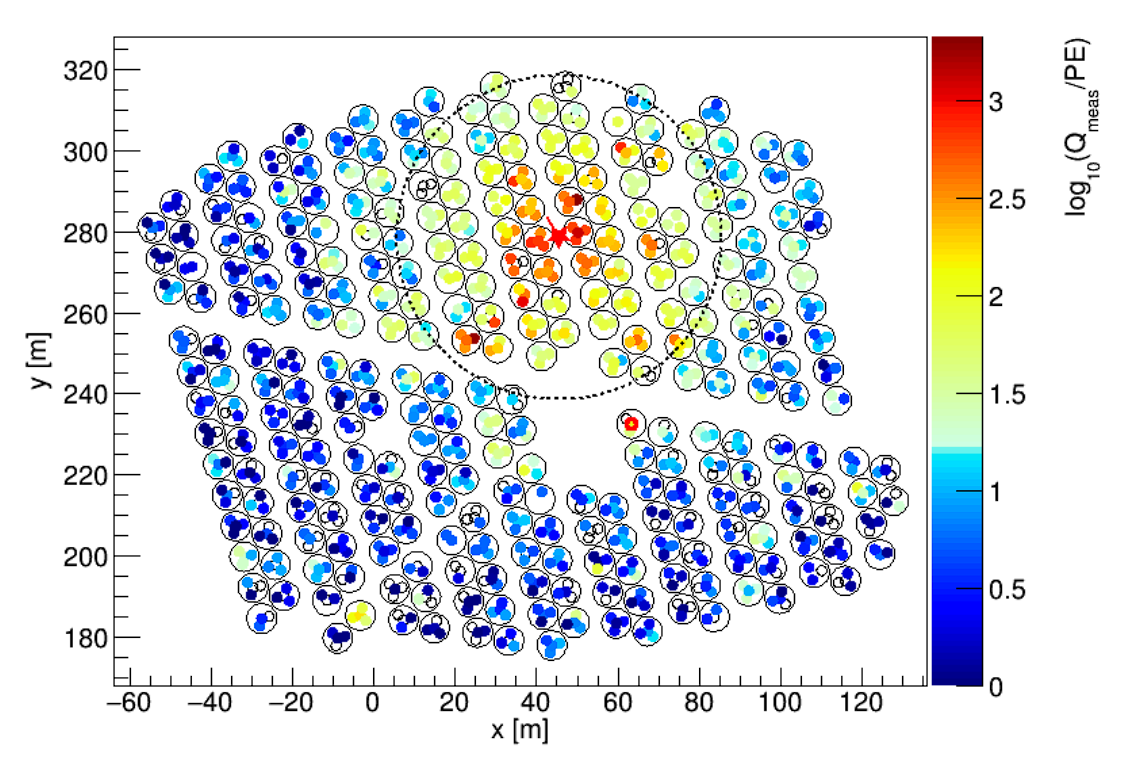
\includegraphics[scale=0.5]{figures/hawc/core_fitting.png}
    }
    \caption{\todo{pulled for thesis}. Charge deposited in each PMT for a reconstructed gamma-ray event. Each large circle represents a WCD and each of the 4 smaller circles within represent a PMT. The color scale represents the amount of charge deposited in each PMT. The red star in the center of the dashed circle shows the location of the shower core fit by the SFCF algorithm. \cite{Abeysekara_2017}}
    \label{fig:core_fitter}
\end{figure}

The chosen functional form for the Super Fast Core Fit (SFCF) algorithm is a simplified version of a modified Nishimura-Kamata-Greisen (NKG) function \cite{cosmic_ray_shape}, selected for its computational efficiency which is essential for rapid fitting of air shower cores. The SFCF form allows numerical minimization to converge more quickly due to the function's simplicity, the analytical computation of its derivatives, and the absence of a pole at the core location.

Figure 2 provides a visualization of a recorded event, with the plot depicting the charge recorded by each PMT as a function of the distance to the reconstructed shower core. The caption explains the plot details, including the reconstructed arrival coordinates and data acquisition run information, and also mentions variables relevant for gamma/hadron separation, as discussed in Section 4.3.1.

Through the application of the SFCF, core locations can be identified with a median error of approximately 2 meters for large events and about 4 meters for smaller ones, assuming the gamma-ray event core impacts directly upon the HAWC detector array. It is noted that as the core's distance from the array increases, the precision in locating the core diminishes, highlighting the importance of proximity in the accuracy of core reconstruction.


%$$$$$$$$$$$$$$$$$$$$$$$$$$$$$$$$$$$$$$$$$$$$$$$$$$$$$$$$$$$$$$$$$$$$$$$$$$$$$$$$$$$%
\subsection{Angle Reconstruction}
%$$$$$$$$$$$$$$$$$$$$$$$$$$$$$$$$$$$$$$$$$$$$$$$$$$$$$$$$$$$$$$$$$$$$$$$$$$$$$$$$$$$%

%$$$$$$$$$$$$$$$$$$$$$$$$$$$$$$$$$$$$$$$$$$$$$$$$$$$$$$$$$$$$$$$$$$$$$$$$$$$$$$$$$$$%
\subsection{\textit{f}-hit Energy Estimation}
%$$$$$$$$$$$$$$$$$$$$$$$$$$$$$$$$$$$$$$$$$$$$$$$$$$$$$$$$$$$$$$$$$$$$$$$$$$$$$$$$$$$%

%$$$$$$$$$$$$$$$$$$$$$$$$$$$$$$$$$$$$$$$$$$$$$$$$$$$$$$$$$$$$$$$$$$$$$$$$$$$$$$$$$$$%
\subsection{Neural Network Energy Estimation}
%$$$$$$$$$$$$$$$$$$$$$$$$$$$$$$$$$$$$$$$$$$$$$$$$$$$$$$$$$$$$$$$$$$$$$$$$$$$$$$$$$$$%

%$$$$$$$$$$$$$$$$$$$$$$$$$$$$$$$$$$$$$$$$$$$$$$$$$$$$$$$$$$$$$$$$$$$$$$$$$$$$$$$$$$$%
\subsection{G/H Discrimination}
%$$$$$$$$$$$$$$$$$$$$$$$$$$$$$$$$$$$$$$$$$$$$$$$$$$$$$$$$$$$$$$$$$$$$$$$$$$$$$$$$$$$%
%-----------------------------------------------------------------------------------%
\section{Remote Monitoring}
%-----------------------------------------------------------------------------------%

%$$$$$$$$$$$$$$$$$$$$$$$$$$$$$$$$$$$$$$$$$$$$$$$$$$$$$$$$$$$$$$$$$$$$$$$$$$$$$$$$$$$%
\subsection{ATHENA Database}
%$$$$$$$$$$$$$$$$$$$$$$$$$$$$$$$$$$$$$$$$$$$$$$$$$$$$$$$$$$$$$$$$$$$$$$$$$$$$$$$$$$$%

%$$$$$$$$$$$$$$$$$$$$$$$$$$$$$$$$$$$$$$$$$$$$$$$$$$$$$$$$$$$$$$$$$$$$$$$$$$$$$$$$$$$%
\subsection{HOMER}
%$$$$$$$$$$$$$$$$$$$$$$$$$$$$$$$$$$$$$$$$$$$$$$$$$$$$$$$$$$$$$$$$$$$$$$$$$$$$$$$$$$$%
